\documentclass[thesis.tex]{subfiles}

\begin{document}
\chapter{Survival analysis with perfect testing} \label{perf-test}

This chapter aims to estimate the duration of SARS-CoV-2 PCR positivity from CIS data if perfect testing can be assumed (\ie: no misclassification bias).
I take a survival analysis approach, considering that neither the start nor end time of positivity are known exactly (double interval censoring) and that infections may be missed (truncation), explained in the following paragraphs.
Through a simulation study, I show the applicability of these methods.
However, application in reality must account for misclassification bias, the subject of the following chapter.

\section{Problem description and approach}\label{perf-test:sec:data}

Consider a series of tests on the same individuals (longitudinal data), where some individuals have a series of positive tests.
We wish to estimate the distribution of time for which an individual is positive for.
An individual could have multiple infections, in which case define \emph{infection episodes}, corresponding to a single infection event.

I define an individual as \emph{detectable} if they would test positive if tested, in the absence of misclassification error (which is dealt with in \autoref{imperf-test}).
The episode's \emph{duration of positivity} is the number of days that they are detectable for; I use time discretised to days, therefore, the duration is at least 1 day.
Note that the relationship between positivity (\ie the result of a PCR test) and infectiousness (\ie an individual's ability to pass on the virus) is complex, \todo{ref for PCR pos vs infectiousness} and beyond the scope of this thesis.

An episode is \emph{detected} when they test positive at least once, if this occurs; episode $i$ is detected at time $t$ if and only if: $i$ is detectable at $t$, $i$ is tested at $t$, and the test returns positive (a false negative does not occur).

I utilise survival analysis for analysing this data.
Survival analysis is the area of statistics concerned with estimating the distribution of the times between events.
It is broadly applicable to many domains, such as the time-to-failure for a mechanical system or the effect of a treatment on time spent in hospital.
In the context of this thesis, the distribution to estimate is that of duration of positivity.
The \emph{initiating event} is when the duration starts, \ie becoming detectable.
The \emph{terminating event} is when the duration starts, \ie becoming no longer detectable.

The reason for this approach, over modelling biomarkers (as in \autoref{ATACCC}) is due to two factors.
First, the large sample size in CIS means that approaches where the number of parameters scales with the number of observed infections (as it does with random effect based approaches) would be computationally challenging; this challenge is compounded by the data being stored in a trusted research environment limiting the computational power and tools available.
Second, the data is coarse with most episodes having only a single positive test; therefore, the trajectory of the viral load would not be well-identified in an individual.
Combined, these factors outweighed the downside of survival analysis only considering the binary outcome (\ie positive or negative) or the test rather than the additional information on the viral load.

The methods in this chapter deal with modelling two elements of the data-generating process, double interval censoring and truncation.
False negatives are not dealt with and left to \autoref{imperf-test}.

Double interval censoring is a special case of censoring, a common and well-studied challenge encountered when dealing with survival data.
An event is \emph{censored} if the time of the event can only be bounded; it is \emph{left censored} if it is known to occur before a certain time, \emph{right censored} if it is known to occur after a certain time, and \emph{interval censored} if it is known to occur within an interval.
Interval censoring arises in CIS because we only observe the change from being not detectable (\ie: negative) at one test, to detectable (\ie: positive) at the following test and vice versa; \textcite{bogaertsSurvival} review many statistical methods applicable to interval censoring (see \autoref{perf-test:fig:double-interval-censor}).
\emph{Double censoring} means that both the originating and terminating event are censored, and is also a well-studied problem, reviewed by \textcite{sunStatisticala}.
In CIS, we have \emph{double interval censoring} meaning that both the initiating and the terminating events are interval censored.
\begin{figure}
  \centering 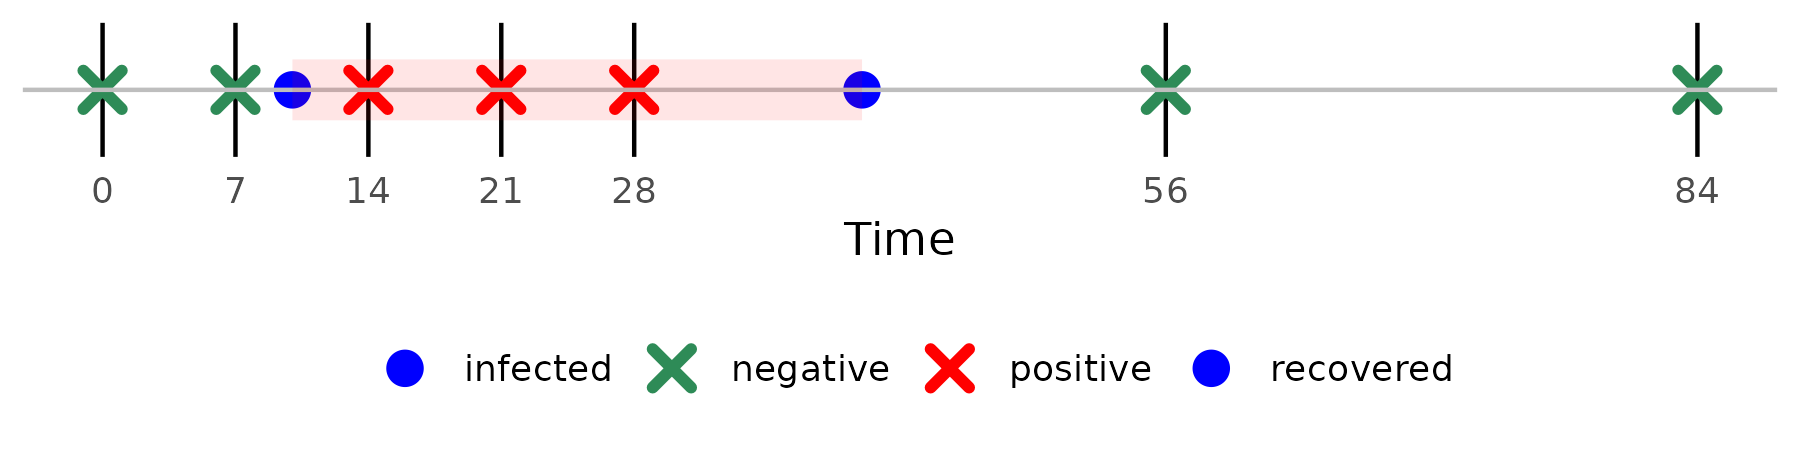
\includegraphics{cis-perfect-testing/double-interval-censor}
  \caption{Episodes data in CIS is double interval censored, meaning that both the start and end of the episode are only known up to an interval. Demonstrated here by a participant who transitions negative at time 7 to positive at time 14, bounding the start of the episode; similarly, the transition positive at time 28 to negative at time 56 bounds the end of the episode. \label{perf-test:fig:double-interval-censor}}
\end{figure}

Interval censoring is a well-studied area in the biostatistics and broader statistical literature\todo{interval censoring refs}.
Double interval censoring is less frequent, although has been considered previously\todo{double interval censoring refs}.

The second element is truncation.
Truncation occurs because we do not observe some episodes: an episode can occur between tests and hence the episode is never detected (see \autoref{perf-test:fig:truncation}).
We do not know how many infections we do not detect.
Failure to model truncation will lead to estimating too long durations because the detected episodes are a biased sample with a longer duration.
To see why they are shorter, consider the undetected infection in the bottom of \autoref{perf-test:fig:truncation}.
This individual was infected at time 33 for 10 days.
If instead there infection was 24 days (or longer), the individual would still have been detectable at their next test, and therefore would have been detected.

Truncation is a large problem when individuals move to the infrequent testing schedule within CIS.
Consider that, based on the estimates in \autoref{ATACCC}, the median length of an episode is 14 days \todo{check this number} we would not expect many episodes to last the 28 days that can occur between tests.
\begin{figure}
  \centering 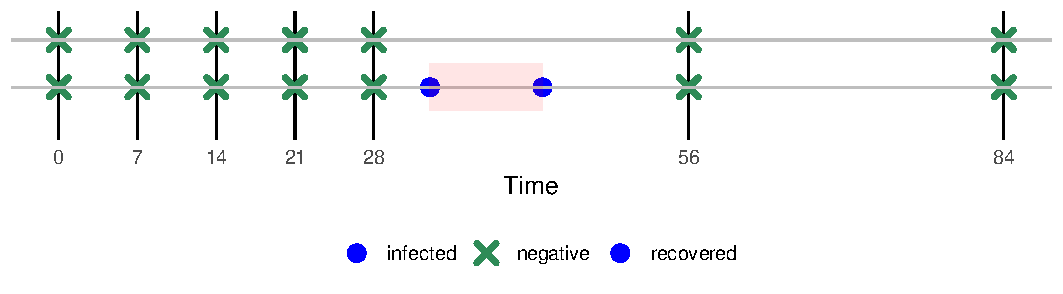
\includegraphics{cis-perfect-testing/truncation}
  \caption{Episodes data in CIS is truncated, meaning that an unknown number of infections are never detected. Consider the two individuals shown here: we collect identical data for them (a series of negative tests) yet the top individual was never infected and the bottom individual was. See the main text for why this is an issue. \label{perf-test:fig:truncation}}
\end{figure}

This combination of censoring and truncation are rarely encountered in biomedical data\todo{refs to combining double interval censoring with truncation}. 

I use the CIS data described in \autoref{intro:sec:cis}, with positive tests heuristically divided into episodes.
Prior work categorised a series of positive tests within the same individual CIS were heuristically categorised into episodes (see \autoref{episode-def}).

I filter the episodes as follows.
\begin{itemize}
\item
  The first positive in the episode occurred between 16th Oct 2020 and
  5th Dec 2020 inclusive.
\item
  The individual had recorded a negative test prior to their episode
  beginning (this could have happened at any time, including prior to
  16th Oct).
\item
  A negative test to end the episode (\ie: following the final positive in the episode) has been recorded.
\end{itemize}

\todo[inline]{Descriptive analyses of the data here}

\section{Modelling the duration}\label{perf-test:sec:model}
Now I develop a model accounting for double interval censoring and truncation, building on prior work in both biomedical and bird nesting studies.
The arbitrary nature of truncation in CIS, where each individual has a unique truncation pattern and is neither simple left nor right truncation, has not previously been explored in the literature.
Furthermore, I explore a Bayesian framework where the amount of explicit data augmentation is limited allowing the method to scale to the large number of episodes present in CIS without requiring vast computing resources (such as a high-performance cluster).
Only limited resources are unavailable within the secure research service (SRS, a form of trusted research environment) where the CIS data is held.
Therefore, unlike most Bayesian methods (e.g.: \textcite{heBayesiana}, \textcite{heBayesian}, and \textcite{caoModeling}) we avoid augmenting the data with unobserved times of infection or any information on the truncated infections; this is due to the large number of infections (>4000 in the time period considered) making this approach computationally expensive.

The individual model considers only individuals with observed (\ie, not truncated) episodes.
This approach is similar to methods used in previous studies, such as \textcite{heiseyModelling}, \textcite{dempsterMaximum}, and \textcite{turnbullEmpirical}.
The conceptual approach here is to form a cohort of individuals for which we observe at least one positive test, and then consider a study which had only enrolled these individuals.
The modelling approach then corrects for this selection bias.

In contrast, the total model also takes into account data from individuals without any observed episodes.
These individuals may have truncated episodes or may not have been infected at all. This approach utilises their test times to estimate the probability of truncated infections, ultimately providing an interpretable estimate of the number of truncated episodes in the cohort.

\subsection{Notation and assumptions}
\todo[inline]{Some of this will possibly be defined elsewhere, such as in the introduction where CIS is introduced}
\begin{itemize}
\item
  Time is discrete: $1, \dots, T$.
\item
  We observe $n_a$ episodes of infection, indexed by $i$.
\item
  The $i$ in which episode $i$ occurs is tested at times
  $t_i = \{ t_{i,1}, \dots, t_{i,m_i} \}$.
\item
  Each observed episode has an unknown start of infection time $b_i$
  and end of infection time $e_i$ (the first and last day that the
  individual would test positive due to this episode respectively).
  These are realisations of the random variables $B_i$ and $E_i$
  respectively.
\item
  The duration of the infection is the number of days for which an
  individual tests positive, $D_i = E_i - B_i + 1$.
\item
  We assume that, for all episodes $i$, $D_i$ is iid and independent
  of the time of the infection. Define the survival function
  $\prob(D_i \geq t \mid B_i = b, \theta) = \prob(D_i \geq t \mid \theta) = S_\theta(t)$,
  where $\theta$ are the parameters controlling the survival
  distribution (the discussion in this document is valid regardless of
  the model specified for $S_\theta$ and hence we consider $\theta$
  as an arbitrary vector of parameters).
\item
  The beginning of episode $i$ is known to occur in the interval
  $[l_i^{(b)}, r_i^{(b)}]$, and similarly for the end of the infection
  in $[l_i^{(e)}, r_i^{(e)}]$.
\item
  $y_i(t)$ for $t \in t_i$ is a binary indicator giving the test
  result for individual $i$ at time $t$. Under the perfect testing
  assumption, $y_i(t) = 1$ if and only if $b_i \leq t \leq e_i$.
\item
  Throughout, the convention that lower-case letters are realisations of
  upper-case random variables is used.
\end{itemize}


\subsection{Individual model}\label{perf-test:sec:individual-model}

\subsubsection{Likelihood}\label{perf-test:sec:likelihood}

Episode $i$ can be fully characterised by the pair $(b_i, e_i)$ of
start and end dates of the episode, which belong to the state space
$T \times T$. If the individual in which the episode occurs is tested
between $b_i$ and $e_i$ (inclusive), then we observe the episode,
otherwise it is truncated. For the $i$th episode that we observed, we
consider there is an unknown number, $n_{it}$, where $(b, e)$ are
drawn from the same distribution as those that lead to episode $i$,
and occur in an (imagined) individual identical to $i$, but were
truncated. Episodes are also truncated if there is no negative test
prior to their start, that is, the individual the episode occurred in
had no tests before $b_i$. The truncated episodes are often referred
to as the ``ghosts'' of $i$.

Formally (and following \textcite{heiseyModelling}), we
define three sets which partition the space of possible infection and
recovery (\ie: are strict subsets of $T \times T$) given the
observations associated with episode $i$ (graphically shown in Figure
\ref{perf-test:fig:partitionSpace}). Each episode, whether observed or not, must
fall into one of these three classes with a probability that is a
function of $\theta$ (see section \ref{perf-test:sec:likelihood}).

\begin{itemize}
\item
  Admissible episodes, $\alpha_i$, which have an infection and
  recovery time within their respective intervals observed.
  $n_{ia} =1$ of these occurred, each with probability
  $p_{ia} = \prob((b, e) \in \alpha_i \mid \theta)$.
\item
  Truncated episodes, $\Omega_i^C$, which have an infection and
  recovery time such that they would not have tested positive. An
  unknown number, $n_{it}$ of these observed, each with probability
  $p_{it} = \prob((b, e) \in \Omega^C_i \mid \theta)$.
\item
  Inadmissible episodes, $\beta_i$, which do not have an infection and
  recovery time within their respective intervals but would have been
  observed (not truncated). This is all remaining episodes not in the
  previous sets. $n_{iu} = 0$ of these occurred, where they would have
  occurred with probability
  $p_{iu} = \prob((b, e) \in \beta_i \mid \theta)$.
\end{itemize}

The untruncated region (where we could have observed an episode) is
$\Omega_i = \alpha_i \cup \beta_i$ (the notation here is used for
consistency with \textcite{heiseyModelling}), and is the
complement of $\Omega^C_i$.

\begin{figure}
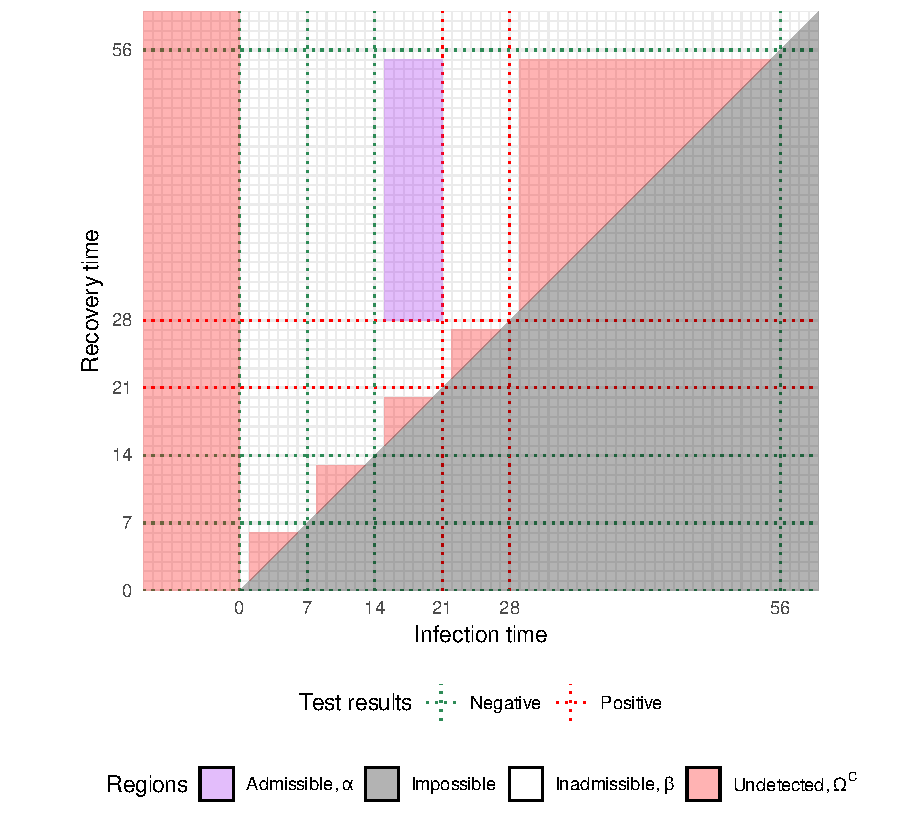
\includegraphics[width=\textwidth]{cis-perfect-testing/regions_diag}
\caption{Admissible, $\alpha_i$, inadmissible, $\beta_i$ and
untruncated, $\Omega_i^C$ regions for an episode $i$ in an
individual whose first test was at time 0 and negative, with subsequent
negative tests at times 7, 14, and 56, and positive tests at times 21
and 28. Purple region is $\alpha_i$, orange region (which includes all
negative infection times) is $\Omega_i^C$ and unshaded region is
$\beta_i$.\label{perf-test:fig:partitionSpace}}
\end{figure}

These three classes span all possible episodes and are mutually
exclusive, and hence the total number of episodes,
$n_i = n_{ia} + n_{iu} + n_{it}$, and
$p_{ia} + p_{iu} + p_{it} = 1$.

Episode $i$ and its ghosts independently occur belong to one of these
classes. Therefore, conditional on $n_i$, the number of episodes in
each class (that is, the counts $n_{ia}, n_{iu}, n_{it}$) are
distributed multinomially. Hence:
\begin{align}
&p(n_{ia} = 1, n_{iu} = 0, n_{it} = n_i - 1 \mid n_i, \theta) \\
&= \frac{n_i!}{n_{ia}! n_{iu}! (n_i- n_{ia} - n_{it})!} p_{ia}^{n_{ia}} p_{ua}^{n_{ia}} p_{it}^{n_i- n_{ia} - n_{it}} \\
&= \frac{n_i!}{(n_i-1)!} p_{ia} p_{it}^{n_i- 1} &\text{as $n_{ia} = 1$ and $n_{iu} = 0$}\\
&= n_i p_{ia} p_{it}^{n_i- 1}
\end{align}

The posterior we are interested in is
$p(\theta \mid n_{ia} = 1, n_{iu} = 0, \dots, n_{n_a,a} = 1, n_{n_a,u} = 0)$,
where $\theta$ are the parameters governing the survival distribution
and hence allow derivation of the $p$s.
\begin{align}
&p(\theta \mid n_{ia} = 1, n_{iu} = 0, \dots, n_{n_a,a} = 1, n_{n_a,u} = 0) \\
&\propto p(\theta) \prod_{i=1}^{n_a} p(n_{ia} = 1, n_{iu} = 0 \mid \theta) \\
&= p(\theta) \prod_{i=1}^{n_a} \sum_{n_i=1}^\infty p(n_{ia} = 1, n_{iu} = 0, n_{it} = n_i - 1 \mid \theta, n_i) p(n_i \mid \theta) \\
&= p(\theta) \prod_{i=1}^{n_a} \sum_{n_i=1}^\infty n_i p_{ia} p_{it}^{n_i- 1} p(n_i) \\
&= p(\theta) \prod_{i=1}^{n_a} p_{ia} \sum_{n_i=1}^\infty n_i p_{it}^{n_i- 1} p(n_i)
\end{align}
where the last line follows by assuming prior independence.

In the remainder of the section, we derive the expressions for $p_{ia}$ and
$p_{it}$ in terms of the data, and analytical solutions for the sum
under different priors.

First, I derive an analytical solution to $\sum_{n_i=1}^\infty n_i p_{it}^{n_i- 1} p(n_i)$ under two different assumptions for $p(n_i)$.
First, we consider the improper prior $p(n_i) \propto 1/n_i$, this prior has several attractive properties.
Then, we consider a negative binomial distribution (which includes the geometric and Poisson distributions as a special and limiting case respectively).

The prior $p(n_i) \propto 1/n_i$ means that the model coincides with the frequentist conditional likelihood approach, up to the priors on other parameters~\cites[section 4.2]{dempsterMaximum}{heiseyModelling}[section 8.7.5]{gelmanBayesian}.
Furthermore, this is the reference prior for this quantity\autocite{heBayesiana}.
Under this prior,
$\sum_{n_i=1}^\infty n_i p_{it}^{n_i- 1} p(n_i) \propto \sum_{n_i=1}^\infty p_{it}^{n_i-1} = 1/(1-p_{it})$.
% (\protect\hyperlink{ref-dempsterMaximum}{Dempster, Laird, and
% Rubin} (\protect\hyperlink{ref-dempsterMaximum}{1977}) section 4.2;
% \protect\hyperlink{ref-heiseyModelling}{Heisey and Nordheim}
% (\protect\hyperlink{ref-heiseyModelling}{1995});
% \protect\hyperlink{ref-gelmanBayesian}{Gelman et al.}
% (\protect\hyperlink{ref-gelmanBayesian}{2013}) section 8.7.5)

Now consider $N_i \sim \text{NegBin}(\mu, r)$ using the
mean/dispersion parameterisation of the negative binomial. Equivalently:
\begin{align}
N_i \mid \lambda &\sim \text{Poisson}(\lambda) \\
\lambda &\sim \text{Gamma}(a, b)
\end{align}
where $b = r / \mu$ and $a = r$.
Hence:
\begin{align}
\sum_{n_i=1}^\infty n_i p_{it}^{n_i- 1} p(n_i) 
&= \int \sum_{n_i=1}^\infty n_i p_{it}^{n_i- 1} p(n_i \mid \lambda) p(\lambda) d\lambda \\
&= \int \sum_{n_i=1}^\infty n_i p_{it}^{n_i- 1} \frac{\lambda^{n_i} e^{-\lambda}}{n_i!} p(\lambda) d\lambda \\
&= \int e^{-\lambda} \sum_{n_i=1}^\infty p_{it}^{n_i- 1} \frac{\lambda^{n_i-1}\lambda }{(n_i-1)!} p(\lambda) d\lambda \\
&= \int e^{-\lambda} \lambda p(\lambda) \sum_{n_t=0}^\infty p_{it}^{n_t} \frac{\lambda^{n_t} }{n_t!} d\lambda &n_t = n_i - 1 \\
&= \int e^{-\lambda} \lambda p(\lambda) e^{p_{it}\lambda} d\lambda &\text{Poisson pmf} \\
&= \int e^{\lambda (p_{it} - 1)} \lambda p(\lambda) d\lambda \\
&= \int e^{\lambda (p_{it} - 1)} \frac{b^a}{\Gamma(a)} \lambda^{a-1} e^{-b\lambda} \lambda d\lambda \\
&= \frac{\Gamma(a+1)b^a}{\Gamma(a) (b+1-p_{it})^{a+1}} \\ 
  &\; \times \int \frac{(b+1-p_{it})^{a+1}}{\Gamma(a+1)} \\
  &\; \lambda^{(a+1)-1} e^{-(b+1-p_{it})\lambda} d\lambda \\
&= \frac{\Gamma(a+1)b^a}{\Gamma(a) (b+1-p_{it})^{a+1}} &\text{as gamma pdf} \\
&\propto (b+1-p_{it})^{-(a+1)} \\
&= (r/\mu+1-p_{it})^{-(r+1)} \\
&\propto (r+\mu (1-p_{it}))^{-(r+1)}
\end{align}
Note that $r=0$ recovers the previous derivation (up to
proportionality).

The above allows us to sample from the posterior without needing to
sample the $n_i$s. This is convenient because there are as many
$n_i$s as episodes observed and hence is computationally costly to
sample. Furthermore, each $n_i$ is a discrete parameter, and hence
cannot be sampled within the current Stan implementation.

Having estimated the posterior of the other parameters, we might want to
consider the posterior of $n_i$ (normally for diagnostic or model
debugging purposes), which we can sample from the full conditional.
Specifically, for each posterior sample of $\theta$, we sample one
draw from $n_i \mid \theta, y$ where $y$ represents all the data.

Due to the conditional independence of the $n_i$s, we find that:
\begin{align}
&p(n_i \mid \theta, n_{ia} = 1, n_{iu} = 0) \\
&\propto p(n_{ia} = 1, n_{iu} = 0, n_{it} = n_i - 1 \mid n_i, p_{iu}, p_{ia}, p_{it}) p(n_i) \\
&\propto n_i p_{it}^{n_i- 1} p(n_i)
\end{align}
With the prior, $p(n_i) \propto 1/n_i$ then this is a geometric
distribution with parameter $1 - p_{it}$. With a negative binomial
prior, we have:
\begin{align}
n_i p_{it}^{n_i- 1} p(n_i)
&\propto n_i p_{it}^{n_i- 1} \frac{\Gamma(r + n_i)}{n_i!} \left( \frac{\mu}{r+\mu} \right)^{n_i} \\
&\propto \frac{\Gamma((r + 1) + (n_i - 1))}{(n_i-1)!} \left( \frac{\mu p_{it}}{r+\mu} \right)^{n_i-1}
\end{align}
which is a negative binomial pmf with size parameter $r+1$ and
probability parameter $\frac{r + \mu (1 - p_{it})}{r+\mu}$. The mean
of this is
\begin{align}
\frac{(r+1)\mu p_{it}}{r+\mu(1-p_{it})}
\end{align}

Next, I derive $p_{ia}$ and $p_{it}$.

By definition, we have
\begin{align}
p_{ia} &= \prob((b, e) \in \alpha_i) \\
\alpha_i &= \{ (b, e) : l_i^{(b)} \leq b \leq r_i^{(b)} \wedge l_i^{(e)} \leq e \leq r_i^{(e)}\}.
\intertext{Hence:}
p_{ia}
&= \prob \left( l_i^{(b)} \leq B_i \leq r_i^{(b)}, l_i^{(e)} \leq E_i \leq r_i^{(e)} \right) \\
&= \prob \left( l_i^{(e)} \leq E_i \leq r_i^{(e)} \mid l_i^{(b)} \leq B_i \leq r_i^{(b)} \right) \prob \left( l_i^{(b)} \leq B_i \leq r_i^{(b)} \right) \\
&=\sum_{b = l_i^{(l)}}^{r_i^{(b)}} \prob \left( l_i^{(e)} \leq E_i \leq r_i^{(e)} \mid B_i = b \right) \prob \left(B_i = b \right) \\
&=\sum_{b = l_i^{(b)}}^{r_i^{(b)}} \prob \left( l_i^{(e)} - b + 1 \leq D_i \leq r_i^{(e)} - b + 1 \right) \prob \left(B_i = b \right) \\
&=\sum_{b = l_i^{(b)}}^{r_i^{(b)}} \left( S_\theta(l_i^{(e)} - b + 1) - S_\theta(r_i^{(e)} - b + 2) \right) \prob \left(B_i = b \right) \\
&\propto \sum_{b = l_i^{(b)}}^{r_i^{(b)}} \left( S_\theta(l_i^{(e)} - b + 1) - S_\theta(r_i^{(e)} - b + 2) \right)
\end{align}
under the assumption of uniform probability of infection time.

Next, we derive $p_{it} = \prob((b, e) \in \Omega^C_i)$, the probability
that episode $i$ was truncated. A truncated episode means that no test
was performed during the episode or there was no negative test prior to
the episode. Denote by $t_i$ the set of testing times for the
individual in which episode $i$ was observed, and define the time
until the next test on the individual after time $t'$ as:
\begin{align}
t^N_{it} &= \min \{ t' \in t_i : t' \geq t \} - t.
\intertext{Then:}
\Omega^C_i
&= \{ (b, e) : \nexists t \in t_i. b \leq t \leq e \vee b \leq \min(t_i) \} \\
&= \{ (b, e) : e - b < t^N_{ib} \vee b \leq \min(t_i) \}.
\intertext{Hence:}
1 - p_{it}
&= 1 - \prob(E_i - B_i < t_{iB_i}^N \vee B_i \leq \min(t_i)) \\
&= 1 - \prob(E_i - B_i < t_{iB_i}^N \wedge B_i > \min(t_i)) - \prob(B_i \leq \min(t_i)) \\
&= 1 - \sum_{b=\min(t_i) + 1}^T \prob(E_i - b + 1 < t_{ib}^N \mid B_i = b) \prob(B_i = b) \\
  &\; - \sum_{t=1}^{\min(t_i)} \prob(B_i = b)\\
&= 1 - \frac{1}{T} \sum_{b=\min(t_i)+1}^T (1 - S_\theta(t_{ib}^N + 1)) - \frac{\min(t_i)}{T} \\
&= 1 - \frac{T-\min(t_i)}{T} + \frac{1}{T} \sum_{b=\min(t_i)+1}^T S_\theta(t_{ib}^N + 1)) - \frac{\min(t_i)}{T} \\
&= \frac{1}{T} \sum_{b=\min(t_i)+1}^T S_\theta(t_{ib}^N + 1)
\end{align}

\subsubsection{Full posterior}\label{perf-test:sec:full-posterior}

Under the prior $p(n_i) \propto 1/n_i$:
\begin{align}
&p(\theta \mid n_{ia} = 1, n_{iu} = 0, \dots, n_{n_a,a} = 1, n_{n_a,u} = 0) \\
&\propto p(\theta) \prod_{i=1}^{n_a} p_{ia} \sum_{n_i=1}^\infty n_i p_{it}^{n_i- 1} p(n_i) \\
&= p(\theta) \prod_{i=1}^{n_a} \frac{p_{ia}}{1-p_{it}} \\
&\propto p(\theta) \prod_{i=1}^{n_a} \frac{\sum_{b = l_i^{(b)}}^{r_i^{(b)}} \left( S_\theta(r_i^{(e)} - b - 1) - S_\theta(l_i^{(e)} - b - 1) \right)}{\sum_{b=\min(t_i)}^T S_\theta(t_{ib}^N + 1)} \\
\end{align}

Under the prior $N_i \sim \text{NegBinom}(\mu, r)$:
\begin{align}
&p(\theta \mid n_{ia} = 1, n_{iu} = 0, \dots, n_{n_a,a} = 1, n_{n_a,u} = 0) \\
&\propto p(\theta) \prod_{i=1}^{n_a} p_{ia} \sum_{n_i=1}^\infty n_i p_{it}^{n_i- 1} p(n_i) \\
&= p(\theta) \prod_{i=1}^{n_a} \frac{p_{ia}}{(r+\mu (1-p_{it}))^{(r+1)}} \\
&= p(\theta) \prod_{i=1}^{n_a} \frac{\sum_{b=l_i^{(b)}}^{r_i^{(b)}} \left( S_\theta(r_i^{(e)} - b - 1) - S_\theta(l_i^{(e)} - b - 1) \right)}{\left( r+\mu/T \left( \sum_{b=\min(t_i)}^T S_\theta(t_{ib}^N + 1) \right) \right)^{(r+1)}} \\
\end{align}

\subsection{Total model}\label{perf-test:sec:total-model}

We now consider all $N$ individuals in the CIS cohort who have at
least one test during the period of interest, this includes those
without an observed infection, and assume that each is equally likely to
be infected. As before, $i = 1, \dots, n_a$ indexes episodes but now
$j = 1, \dots, N$ indexes individuals. All episodes have an associated
individual, each individual may have any number (including 0) episodes.
Admissible regions are only defined for episodes, and have not changed
from the previous section. The truncated region is defined for each
individual, in addition we consider the combined truncated region which
is episodes that would be truncated without conditioning on which
individual the episode occurs in:
$\Omega^C = \{ (b, e, j) : (b, e) \in \Omega_j^C \}$.

Denote by $n_\text{tot}$ the total number of episodes across all $N$
individuals, regardless of whether they are admissible or truncated (we
know there are no inadmissible episodes by definition).

For any infection, the probability of it being admissible for episode
$i$ is $\frac{1}{N} p_{ia}$. That is, the probability that the
infection occurs in the individual corresponding to the individual in
which episode $i$ ($1/N$ by the assumption that episodes are equally
likely to occur in any of the $N$ individuals) multiplied by the
probability that the episode is admissible for episode $i$ conditional
on it occurring in the relevant individual ($p_{ia}$).

The total number of truncated infections that occur is
$n_t = n_\text{tot} - n_a$. Conditional on an infection occurring in
individual $j$, its probability of being truncated is $p_{jt}$ (as
defined previously). Therefore, the overall probability of an episode
being truncated is $p_t = \frac{1}{N} \sum_{j=1}^N p_{jt}$.

Consider our data as there being one admissible episode for each
observed episode, and all other episodes being truncated. As in the
previous section, conditional on $n_\text{tot}$, we have a multinomial
likelihood.
\begin{align}
p(\text{data} \mid \theta)
&= \sum_{n_\text{tot}=n_a}^\infty p(\text{data} \mid n_\text{tot}, \theta) p(n_\text{tot}) \\
&= \sum_{n_\text{tot}=n_a}^\infty \frac{n_\text{tot}!}{(n_\text{tot}-n_a)!} \left( \prod_{i=1}^{n_a} \frac{1}{N} p_{ia} \right) p_t^{n_\text{tot}-n_a} p(n_\text{tot}) \\
&= \left( \prod_{i=1}^{n_a} \frac{1}{N} p_{ia} \right) \left( \sum_{n_\text{tot}=n_a}^\infty \frac{n_\text{tot}!}{(n_\text{tot}-n_a)!} p_t^{n_\text{tot}-n_a} p(n_\text{tot}) \right) \\
\end{align}

In this case, it would be computationally feasible to augment the data
with $n_\text{tot}$ directly (as it is only a single parameter).
However, implementation is easier if we can use a closed-form for the
sum (as in the previous section) as it allows the use of standard
implementations of NUTS such as Stan, which cannot handle discrete
parameters.

Assuming $N_\text{tot} \sim \text{NegBin}(\mu, r)$:
\begin{align}
&\sum_{n_\text{tot}=n_a}^\infty \frac{n_\text{tot}!}{(n_\text{tot}-n_a)!} p_t^{n_\text{tot}-n_a} p(n_\text{tot}) \\
&= \int \sum_{n_\text{tot}=n_a}^\infty \frac{n_\text{tot}!}{(n_\text{tot}-n_a)!} p_t^{n_\text{tot}-n_a} p(n_\text{tot} \mid \lambda) p(\lambda) d\lambda \\
&= \int \sum_{n_\text{tot}=n_a}^\infty \frac{n_\text{tot}!}{(n_\text{tot}-n_a)!} p_t^{n_\text{tot}-n_a} \frac{\lambda^n_\text{tot} e^{-\lambda}}{n_\text{tot}!} p(\lambda) d\lambda \\
&= \int \sum_{n_\text{tot}=n_a}^\infty \frac{1}{(n_\text{tot}-n_a)!} p_t^{n_\text{tot}-n_a} \lambda^{n_\text{tot}-n_a} \lambda^{n_a} e^{-\lambda} p(\lambda) d\lambda \\
&= \int \lambda^{n_a} e^{-\lambda} p(\lambda) \sum_{n_t=0}^\infty \frac{1}{n_t!} p_t^{n_t} \lambda^{n_t} d\lambda &n_t = n-n_a\\
&= \int \lambda^{n_a} e^{-\lambda} p(\lambda) e^{\lambda p_t} d\lambda \\
&= \int \lambda^{n_a} e^{-\lambda(1 - p_t)} p(\lambda) d\lambda \\
&= \int \lambda^{n_a} e^{-\lambda(1 - p_t)} \frac{b^a}{\Gamma(a)} \lambda^{a-1} e^{-b\lambda} \lambda d\lambda \\
&= \int \frac{b^a}{\Gamma(a)} \lambda^{a+n_a-1} e^{-(b+1-p_t)\lambda} \lambda d\lambda \\
&= \frac{b^a}{\Gamma(a)} \frac{\Gamma(a+n_a)}{(b+1-p_t)^{a+n_a}} \\
&\propto (b+1-p_t)^{-(a+n_a)} \\
&= (r/\mu + 1 - p_t)^{-(r+n_a)} \\
&\propto(r + \mu (1- p_t))^{-(r+n_a)}
\end{align}

Which gives the full posterior density as:
\begin{align}
p(\theta \mid \text{data})
&\propto \frac{p(\theta) \prod_{i=1}^{n_a} p_{ia}}{(r + \mu(1 - p_t))^{r+n_a}}
\end{align}

As before, being able to reconstruct the posterior of $n_\text{tot}$
using its full conditional is useful.
\begin{align}
p(n_\text{tot} \mid \text{data}, \theta)
&\propto p(\text{data} \mid \theta, n_\text{tot}) p(n_\text{tot}) \\
&= \frac{n_\text{tot}!}{(n_\text{tot}-n_a)!} \left( \prod_{i=1}^{n_a} \frac{1}{N} p_{ia} \right) p_t^{n_\text{tot}-n_a} p(n_\text{tot}) \\
&\propto \frac{n_\text{tot}!}{(n_\text{tot}-n_a)!} p_t^{n_\text{tot}} \frac{\Gamma(r + n_\text{tot})}{n_\text{tot}!} \left( \frac{\mu}{r + \mu} \right)^{n_\text{tot}}  \\
&\propto \frac{\Gamma(r + n_\text{tot})}{(n_\text{tot}-n_a)!} \left( \frac{\mu p_t}{r + \mu} \right)^{n_\text{tot}}  \\
&\propto \frac{\Gamma((r + n_a) + (n_\text{tot}- n_a))}{(n_\text{tot}-n_a)!} \left( \frac{\mu p_t}{r + \mu} \right)^{n_\text{tot}-n_a}  \\
\end{align}
which is a negative binomial pmf with size parameter $r + n_a$ and
probability parameter $\frac{r+\mu(1-p_t)}{r+\mu}$.

\section{Parameterisation and priors for the survival function} \label{perf-test:sec:parameters-priors}

\todo[inline]{Section is currently notes: expand into prose which can largely come from previous documents}

In this section, I consider the various parameterisation of the survival function that are available.
This has implications for the choice of prior  it is not possible to be vague on all sensible parameterisations.
Informative priors might also be attractive, and allow the incorporation of the estimates from \autoref{ATACCC}.

Define hazard and survival (maybe this should be done previously?).

The hazard is convenient to use because it is unconstrained except in the interval [0, 1]\todo{ref where been used previously}.
Survival needs to be monotonic.

The main building basis of the priors I propose is the Beta Process\todo{Beta Process refs}.
The Beta Process is...

\subsection{Independent priors}

Traditional uninformative priors, such as Beta(1, 1) or Beta(0.5, 0.5), are unsuitable.

Instead, I propose Beta(0.1, 1.9), linking to previous literature for a point estimate and showing vague figures.

\subsection{Smoothing priors}

\subsection{Informative priors}

ATACCC can be used to provide prior information for the CIS analysis.

Intuition: ATACCC informs early part, CIS informs late part.

Problem: do not believe late part of ATACCC analysis.

First, transform ATACCC analysis into a posterior over survival time.

Second, approximate ATACCC analysis with multivariate normal distribution.
Show that this is a good approximation.

Finally, use a Beta Process to discount some information in ATACCC towards a vague prior (as in the previous section).

\section{Simulation study} \label{perf-test:sec:simulation-study}

\subsection{Setup}

\subsubsection{Testing and infection times}

\subsubsection{Duration of positivity}

We require a ground truth for the distribution giving duration of positivity.
The majority of this distribution is based on \autoref{ATACCC}'s estimates from the ATACCC data.
However, the tail is modified based on Sarah Walker's (unpublished) work based on CIS data.
ATACCC is thought to estimate accurately the majority of the distribution but not the tail due to a small sample size and model uncertainty.
These curves and the combined curve are compared in \autoref{perf-test:fig:duration-dist}.
Individual $i$'s duration of positivity, $d_i$, is then an independent draw from this distribution.

\begin{figure}
  \todo[inline]{Find figure comparing different duration distributions}
  \caption{Comparison of the duration distributions, see main text for details of how each is derived. \label{perf-test:fig:duration-dist}}
\end{figure}

Sarah uses survival analysis to estimate the duration from CIS data.
The initiating event is assumed known as the time the episode was detected.
The final event is assumed interval-censored between the time of the final positive test and the subsequent negative test, or right-censored if a negative test has not yet been observed.
A flexible, spline-based form is assumed for the baseline survival function~\autocite{roystonSTPM,roystonFlexible} with covariates introduced via proportional odds.

We know of two biases introduced from this analysis.
\enquote{There is a bias in estimating the clearance distribution because the analysis used to estimate how long a person stays positive only starts from their first positive test.
Since (most) people will have become positive on an earlier day, this will bias the clearance curves downwards (making the estimates too short).
However, there is another bias due to the survey missing positive episodes entirely if they are short.
This means that our dataset has fewer short positive episodes than in the population as a whole, and that the sample used to run the survival analysis is biased towards people with longer positive episodes.
This will bias the clearance curves upwards (making the estimates too long).}~\autocite{cisMethodsONS}.

To form the duration distribution used in the simulation, we combine these two estimates.
The first 30 days of the distribution is proportional to the ATACCC estimate, with the rest proportional to this CIS-based estimates.
The CIS-based estimates are shifted 3 days in order to make this smooth; this counteracts the above bias of missing the start of the infection (for times above 30 days, the other bias, missing short infections, is negligible).
Denote by $f_A(t)$ the distribution function estimated from ATACCC and $f_C(t)$ that from these CIS-based estimates.
Define:
$$
f_S'(t) = \begin{cases}
	f_A(t) &t \leq 30 \\
	f_C(t-3) &t > 30
\end{cases}
$$
Then the distribution used in the simulation is the normalised version of this: $f_S(t) = f'_S(t)/\sum_i f_S'(i)$.

\subsubsection{Test results and episode summaries}
\todo[inline]{Make notation here consistent with elsewhere}

The first day individual $i$ can be positive is their day of infection, $t_i^\text{onset}$, the last day is $t_i^\text{final} = t_i^\text{onset} + d_i - 1$ where $d_i$ is the duration of positivity for individual $i$.
Outside this period, all tests are negative (\ie: no false positives occur). 
Any test between $t_i^\text{onset}$ and $t_i^\text{final}$ (inclusive) is positive with probability $p_{sens}$ (that is, each test is an independent Bernoulli trial).

Each individual is then summarised into an "episode" (when working with CIS data, the same individual can have multiple episodes due to reinfections, these are split heuristically but a negligible number in the pre-Omicron period and hence ignored within the simulation).
An episode is characterised by:

- The total number of positive tests observed per individual, $n_i^\text{pos}$.
- The time of an individual's first positive test $V'_i$.
- The time of an individual's last negative test prior to $V_i'$, $E'_i$.
- The time of an individual's last positive test, $L_i'$.
- The time of an individual's first negative test after $L_i'$, $R_i'$.

\subsubsection{Restrictions and sample size}

When using the real testing schedules, we then filter the episodes to replicate the process used when working with the CIS data.
First, we discard any episodes where $n_i^\text{pos}=0$ as they are never detected.
We then apply the same criteria as that applied to the modelling dataset (see Section \@ref(design)).
Finally, of those remaining episodes, we select a random subset to match the number of episodes in the simulation to the number of episodes in the modelling cohort.
The last step is required because we infect everyone in the simulation which does not happen in reality.

\subsection{Descriptive analyses of simulated data}

\subsection{Results}

\todo[inline]{Need to decide what exactly to include... There's lots of possible results but need to form some coherent story here!}

\section{Discussion}

\todo[inline]{Add discussion after deciding on results}

\section{Conclusion} \label{perf-test:sec:conclusion}

\listoftodos

\end{document}